\documentclass[aspectratio=169]{beamer}

\mode<presentation>
{
  \usetheme{Madrid}
  \usecolortheme{default}
  \usefonttheme{default}
  \setbeamertemplate{navigation symbols}{}
  \setbeamertemplate{caption}[numbered]
} 

\usepackage[english]{babel}
\usepackage[utf8x]{inputenc}

\usepackage{float}
\usepackage{tikz}
\usetikzlibrary{arrows, fit, calc, shapes, shadows, positioning} % for pgf-umlsd
\usepackage[underline=true,rounded corners=false]{pgf-umlsd}

\title[Alexa unplugged: AI and Privacy]{Alexa unplugged: AI and Privacy}

\author{Maximilian Bachmann\\}

%\institute{\bf}
%\textsc { }

\date{\today}

\begin{document}

\begin{frame}
  \titlepage
\end{frame}





\section{Was macht den Datenschutz im Sprachkontext so wichtig?}
\begin{frame}{Was macht den Datenschutz im Sprachkontext so wichtig?}
\begin{itemize} 
	\item Sprache kann viel über die Emotionen oder den Gemütszustand eines Menschen aussagen
	\item Maschinen können auch mit der Stimme eine Person mit guter Sicherheit identifizieren
	\item Stimme kann nicht verändert werden
\end{itemize}
$\Rightarrow$ Stimme ist ein biometrischen "Abdruck" einer Person (ähnlich wie z.B. Fingerabdrücke, Netzhauterkennung oder Venenkartierung)

$\Rightarrow$ Stimme kann kopiert und manipuliert werden, so dass sie imitiert und die Identität gestohlen werden kann

\end{frame}

\begin{frame}{Was macht den Datenschutz im Sprachkontext so wichtig?}
	\begin{itemize} 
		\item Spracherkennungstechnologie basiert auf maschinellen Lerntechniken, die per Definition Trainingsdaten benötigen
		\item es gibt zwar bereits viele Forschungsarbeiten die sich mit der automatisierten Kennzeichnung beschäftigen, aktuell muss dies allerdings immer noch manuell geschehen
	\end{itemize}
\end{frame}

\begin{frame}{Was macht den Datenschutz im Sprachkontext so wichtig?}
	\begin{figure}
		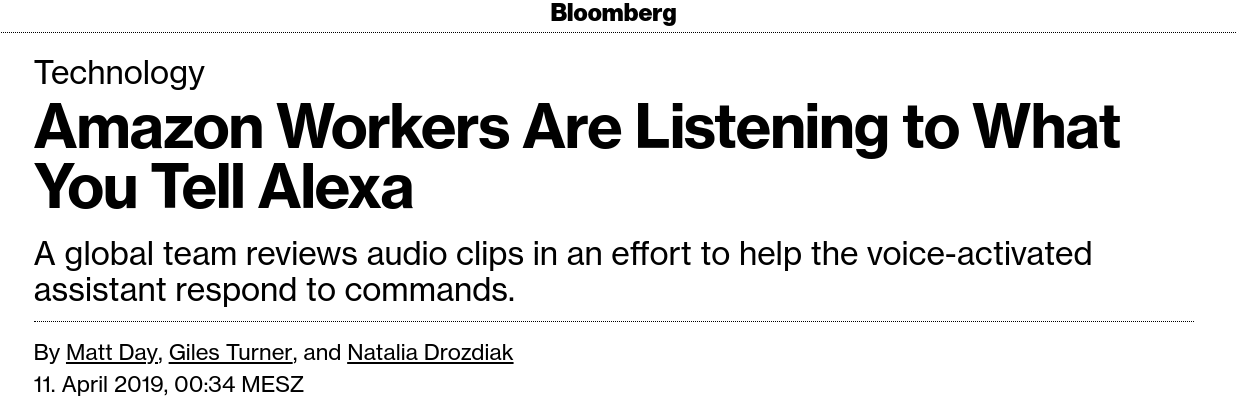
\includegraphics[scale=0.3]{images/alexa-audio-reviews}
	\end{figure}
	\begin{itemize} 
		\item Amazon beschäftigt mehrere Tausend Personen zur Verbesserung von Alexa $\Rightarrow$ Jeder Reviewer kann pro Schicht rund 1000 Aufnahmen kategorisieren
		\item Auch Auswertung von unabsichtlichen Aufnahmen ($\sim$ 10\%)
		\item Es gibt zwar eine Opt Out Möglichkeit, jedoch kein Hinweis auf diese Sprachauswertung in den Nutzungsbedingungen
	\end{itemize}
\end{frame}

\begin{frame}{Was macht den Datenschutz im Sprachkontext so wichtig?}
	\begin{itemize} 
		\item Sprachassistenen von Natur aus invasiv (oft in intimen Kontexten eingesetzt)
		\begin{itemize} 
			\item in der Regel zu Hause auch in Schlaf- und Badezimmern
			\item auch immer mehr in Besprechungsräumen, Fabriken und Autos
		\end{itemize}
	    \item Anwesenheit wird dem unbewussten Beobachter oft nicht mitgeteilt
	    \item Viele Informationen können gesammelt werden ohne, dass dies aktiv bemerkt wird
	    \begin{itemize} 
	    	\item durch unbeabsichtigtes Auslösen (false positive wakeword)
	    	\item andere Informationen abgeleitet aus dem Gebrauch des Sprachassistenten
	    \end{itemize}
	\end{itemize}
\end{frame}

\begin{frame}{Was macht den Datenschutz im Sprachkontext so wichtig?}
	\begin{figure}
		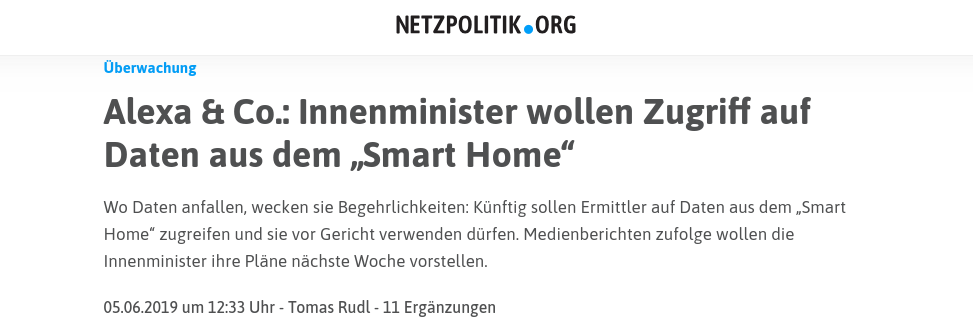
\includegraphics[scale=0.3]{images/alexa-police-access}
	\end{figure}
	\begin{itemize} 
		\item unter dem Argument der Verbrechensbekämpfung gibt es auch in Deutschland immer radikalere Überwachungsgesetze
		\item in den USA müssen entsprechend dem Foreign Intelligence Surveilance (FISA) Act schon länger auch Daten von US Unternehmen wie Amazon die nicht in den USA gespeichert werden an US Nachrichtendienste herausgegeben werden
    \end{itemize}
\end{frame}

\begin{frame}{Was macht den Datenschutz im Sprachkontext so wichtig?}
	\begin{itemize} 
		\item Die Interaktion mit Sprachassistenten wird wesentlich flüssiger je mehr zusätzlichen Informationen über den Geschmack, die Kontakte, die Gewohnheiten usw. der Endbenutzer bekannt ist
	\end{itemize}
    $\Rightarrow$ Es besteht entsprechend der Wunsch der Unternehmer immer mehr private Daten des Nutzer zu erhalten, wobei diese entsprechend wieder großen Spielraum für Missbrauch geben
\end{frame}


\begin{frame}{Was macht den Datenschutz im Sprachkontext so wichtig?}
	Sprachassistenten kombinieren:
	\begin{itemize} 
		\item Daten mit biometrischem Potenzial
		\item Datenintensive Technologie
		\item Anwendungsfälle, die sich auf intime und vertrauliche Bereiche konzentrieren
		\item Verbesserungen, die sich auf das Hinzufügen von Kontexten und das Erlangen von mehr Informationen über Endbenutzer konzentrieren
	\end{itemize}
     $\Rightarrow$ Sprachassistenten bieten ein hohes Potential Bedrohungen der Privatsphäre zu erzeugen, wenn diese nicht im Hinblick auf die Privatsphäre entwickelt werden
\end{frame}


%Privatsphäre vs Datenschutz
\begin{frame}{Leistung vs. Datenschutz}
	Eine häufige Rechtfertigung für die Zentralisierung stellt die Leistung dar. So wird behauptet, dass die Zentralisierung von Endbenutzerdaten erforderlich ist, um die Leistung von Cloud-basierten Assistenten zu maximieren
	\begin{itemize} 
		\item Fehlalarme und Leistungsprobleme zwar vorhanden, hierfür sind aber nicht so enorme Datenmengen notwendig
		\item ab einem bestimmten Punkt verbessert sich die Leistung durch mehr Daten nur noch relativ wenig
		\item optimale Leistung benötigt eine Vielzahl an Daten, aber auch hier sollten die Unternehmen bereits genügend Daten haben
		\item Es gibt Alternativen zu Datensätzen von Endbenutzern die vergleichbare Ergebnisse erzielen (z.B Mozilla Common Voice)
	\end{itemize}
\end{frame}

\begin{frame}{Funktionsweise Sprachassistenten}
	\begin{figure}
		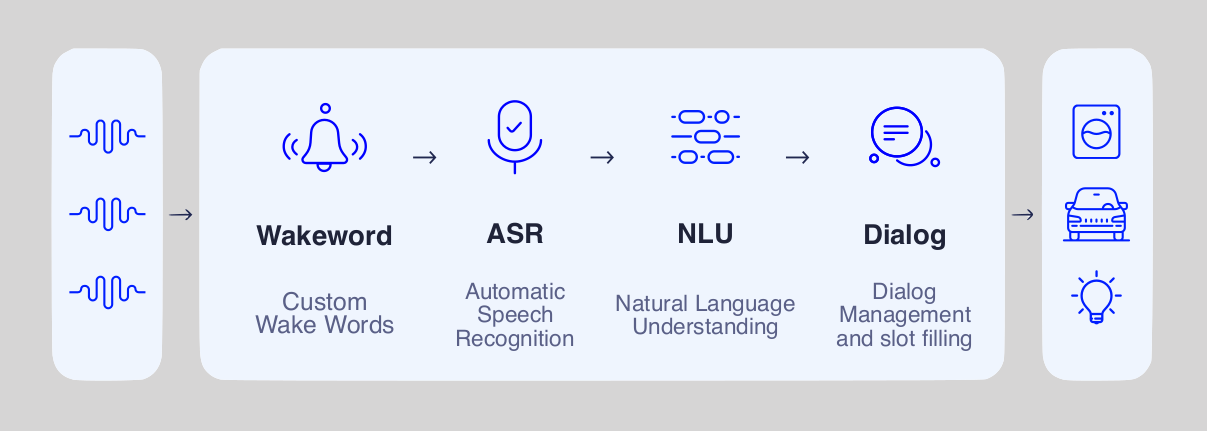
\includegraphics[scale=0.3]{images/assistant}
	\end{figure}
\end{frame}

\begin{frame}{Spracherkennung}
	\begin{figure}
		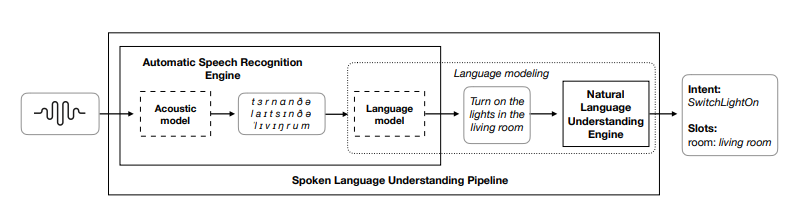
\includegraphics[scale=0.5]{images/spoken-language-understanding}
	\end{figure}
\end{frame}

\begin{frame}{Leistungsbenchmark}
	\begin{figure}
		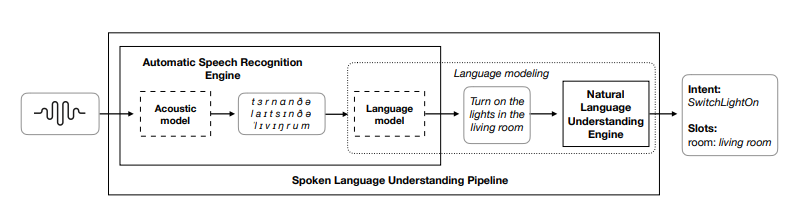
\includegraphics[scale=0.45]{images/spoken-language-understanding}
	\end{figure}
	\begin{itemize}
		\item Akkustisches Modell wandelt raw Audio in Phonem Warscheinlichkeiten um
		\item Sprachmodell wandelt diese in Wörter um
		\item NLU extrahiert strukturierte Daten aus dem gesprochenen Text
	\end{itemize}
\end{frame}

\begin{frame}{Automatic Speech Recognition Engine}
	ASR cloud:
	\begin{itemize}
		\item Spracherkennung auf Basis von großen deep learning Modellen hat sich in den letzten Jahren stark verbessert
		\item entsprechende Modelle für menschliche Parität bestehen aus mehreren neuralen Netzwerken mit jeweil mehreren hundert Millionen Parametern, sowie Sprachmodelle aus mehreren Millionen n-grams
	\end{itemize}
	$\Rightarrow$ Die Größe der Modelle in Verbindung mit der Echtzeitanforderung machen einen Einsatz auf kleinen Geräte unmöglich
\end{frame}

\begin{frame}{Automatic Speech Recognition Engine}
	Ansatz von Snips zur Lösung der Probleme:
	\begin{itemize}
		\item Nutzung von Audioaufnahmen aus öffentlichen oder kommerziellen Quellen
		\item wesentlich kleineres akkustisches Modell
		\item Spezialisierung des Sprachmodells
	\end{itemize}
\end{frame}

\begin{frame}{Leistungsbenchmark}
	\begin{figure}
		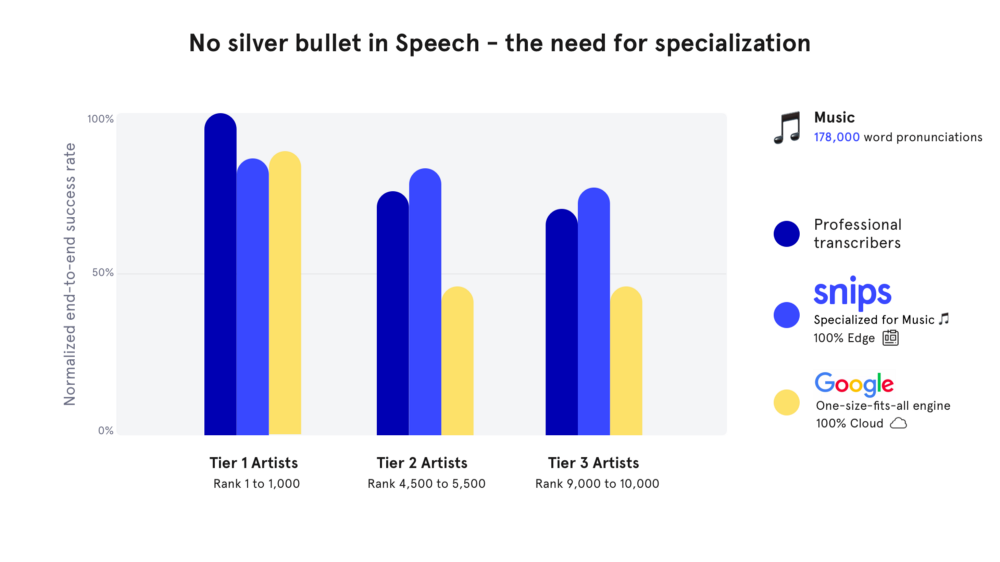
\includegraphics[scale=0.3]{images/benchmark-3}
	\end{figure}
\end{frame}

\section{MQTT}

\begin{frame}{MQTT}

\begin{figure}
	\centering
	\begin{sequencediagram}
		\newthread{client1}{Client 1}
		\tikzstyle{inststyle}+=[below right=-0.85cm and 3cm of client1]
		\newthread[gray]{broker}{Broker}
		\tikzstyle{inststyle}+=[below right=-0.85cm and 3cm of broker]
		\newthread{client2}{Client}

		\mess{client1}{connect}{broker}
		\mess{client2}{connect}{broker}
		\begin{sdblock}{loop}{main loop}
			\mess{client2}{subscribe: 'topic/'}{broker}
			\mess{client1}{publish: 'topic/'}{broker}
			\mess{broker}{publish: 'topic/'}{client2}
		\end{sdblock}
		\mess{client1}{disconnect}{broker}
		\mess{client2}{disconnect}{broker}
	\end{sequencediagram}
	
	\caption{MQTT}
\end{figure}

\end{frame}
%%%%%%%%%%%%%%%
\end{document}
